%!TEX program = xelatex
\documentclass[a4paper, UTF8]{ctexrep}
\usepackage{ctex}
\usepackage{amsmath}
\usepackage{multirow}
\usepackage{amssymb}
\usepackage{graphicx}
\usepackage{geometry}
\usepackage{bm}
\usepackage{subfigure}
\usepackage{float}
\usepackage{array}
\usepackage{makecell}

\renewcommand\thesection{\arabic{section}}

\begin{document}
	\begin{titlepage}
		\centering
		\vspace{6cm}
		\LARGE{\textbf{Deep Learning Homework 2}}\\
		\vspace{4cm}
		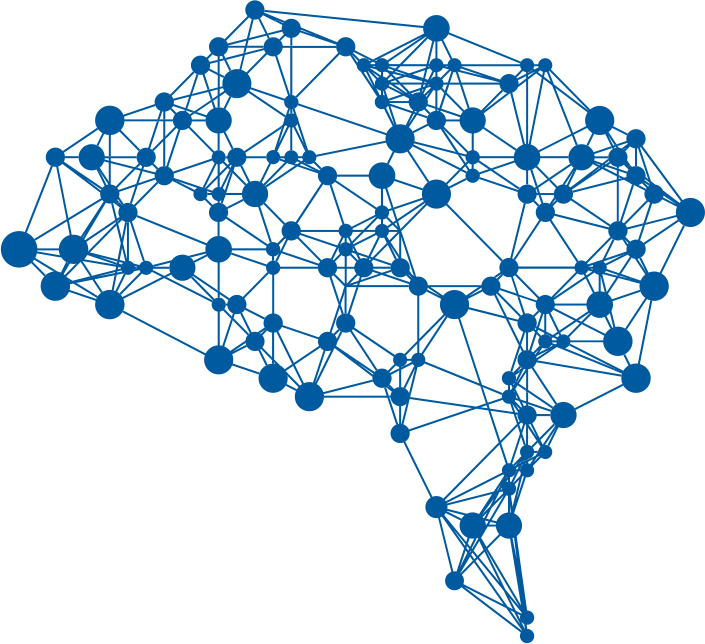
\includegraphics[width=0.8\textwidth]{deepLearning.png}\\
		\vspace{4cm}
		\normalsize{安捷 1601210097}\\
		\normalsize{\today}
	\end{titlepage}
		\section{算法实现简介}
			在这次作业中,为了能够更好的实验不同优化算法的性能及对参数的敏感性,我放弃了上次作业中使用的MLP网络,重新实现了一个有两个卷积层和一个全连接层的CNN,并针对mnist数据集测试了不同优化算法的性能,性能测试主要分为两部分:
			\begin{enumerate}
				\item 对每个算法使用相同的学习率及其他超参数,分别测试算法达到99\%测试准确率的迭代次数,以此来显示算法的性能;
				\item 对每一个算法,分别使用默认学习率或超参数、比默认参数高一个数量级、低一个数量级三组参数分别测试其达到99\%准确率的迭代次数,以此作为衡量算法对学习率或超参数敏感性的指标;
			\end{enumerate}
		\section{算法性能测试}
			\begin{table}[htbp!]
				\centering
				\begin{tabular}{cccc}
					\hline
					算法名称 & 学习率/超参数 & 迭代次数 & 备注 \\
					\hline
					SGD & 0.001 & 4000 &   \\
					SGD with Momentum & 0.001 & 5700 & momentum=0.0005 \\
					SGD with Nesterov Momentum & 0.001 & 5400 & momentum=0.0005 \\
					AdaGrad & 0.001 & 9900 & 未达到99\% \\
					RMSProp & 0.001 & 2500 &   \\
					Adam & 0.001 & 2500 &   \\
					\hline
				\end{tabular}
				\caption{优化算法达到99\%准确率所需迭代次数}
			\end{table}
			从上表中可以看出,在同样的参数设置下,在mnist数据集下使用cnn进行分类,RMSProp和Adam明显具有更好的性能,其余算法的性能较差(性能差的原因有可能因为参数设置不恰当)
			\clearpage
		\section{算法超参数稳定性测试}
			\begin{table}[htbp!]
				\centering
				\begin{tabular}{cccc}
					\hline
					算法名称 & 学习率/超参数 & 迭代次数 & 备注 \\
					\hline
					SGD & 0.01 & 9900 & 未收敛  \\
					SGD & 0.0001 & 9900 & 达到98\% \\
					SGD with Momentum & 0.01 & 未收敛 & momentum=0.0005 \\
					SGD with Momentum & 0.0001 & 达到98\% & momentum=0.0005 \\
					SGD with Momentum & 0.001 & 6100 & momentum=0.005 \\
					SGD with Momentum & 0.001 & 未收敛 & momentum=0.00005 \\
					SGD with Nesterov Momentum & 0.01 & 未收敛 & momentum=0.0005 \\
					SGD with Nesterov Momentum & 0.0001 & 达到98\% & momentum=0.0005 \\
					SGD with Nesterov Momentum & 0.001 & 4300 & momentum=0.005 \\
					SGD with Nesterov Momentum & 0.001 & 未收敛 & momentum=0.00005 \\
					AdaGrad & 0.01 & 不收敛 & 未达到99\% \\
					AdaGrad & 0.0001 & 9900 & 达到91\% \\
					RMSProp & 0.01 & 未收敛 &   \\
					RMSProp & 0.0001 & 8300 &   \\
					Adam & 0.01 & 不收敛 &   \\
					Adam & 0.0001 & 7200 &   \\
					\hline
				\end{tabular}
				\caption{算法不同超参数下固定迭代次数达到的准确率}
			\end{table}
			从上表可以看出,不同的算法对于参数都有很大的敏感性,无论是学习率还是动量参数,都会影响最终的结果,比较显著的但是又不言自明的特点是,过小的参数会导致算法的收敛速度变慢,过大的参数会使得算法不收敛。
			\clearpage

    \section{代码运行环境及测试平台信息}
      \begin{table}[htbp!]
        \centering
        \begin{tabular}{l}
          \hline
          Python Version: 3.6.0 \\
          Tensorflow Version: tensorflow-gpu-1.0.1 \\
          CUDA Version: 8.0 \\
          OS: Arch Linux \\
          Kernel: x86\_64 Linux 4.10.4-1-ARCH \\
          CPU: Intel Core i7-6700K @ 8x 4.2GHz \\
          GPU: GeForce GTX 1060 6GB \\
          RAM: 16003MiB \\
          \hline
        \end{tabular}
        \caption{代码运行环境及测试环境表}
      \end{table}
      在没有NVIDIA\ GPU及CUDA支持的环境下代码依然可以运行,只是速度较慢
    \section{总结}
      通过这次作业,我学习了tensorflow实现cnn的基本方法,同时尝试使用了不同的优化算法来学习参数,发现了参数对算法结果的巨大影响,明白了调参的重要性。
\end{document}
